% Figure 2 uses the externally supplied SVG/PDF artwork.
% Required packages:
% \usepackage{tikz}
% \usetikzlibrary{arrows.meta,positioning,fit,backgrounds}
% \usepackage{xcolor}
% \usepackage{graphicx}

\begin{figure*}[t]
\centering
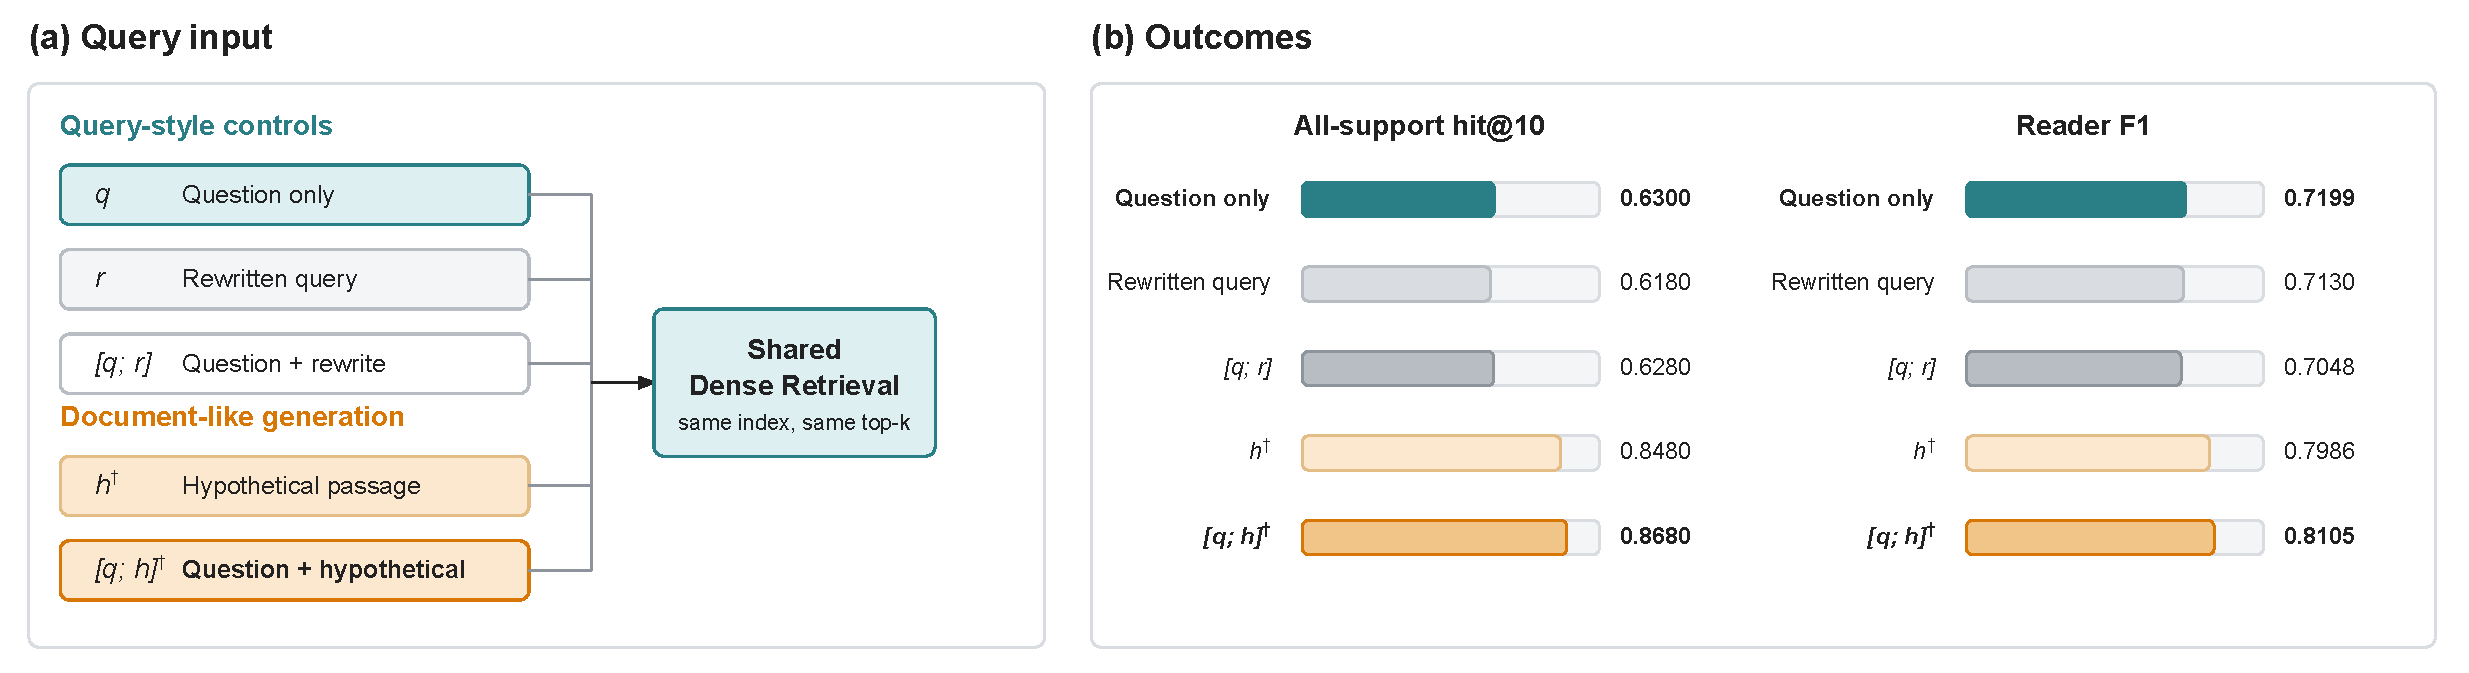
\includegraphics[width=\textwidth]{../figures/figure2.pdf}
\iffalse
\resizebox{\textwidth}{!}{%
\begin{tikzpicture}[
    font=\sffamily\footnotesize,
    input/.style={draw=black!34, rounded corners=2pt, fill=white, align=left,
                  text width=42mm, minimum height=7.2mm, inner sep=3pt},
    inputemph/.style={input, draw=teal!55!black, line width=0.85pt, fill=teal!5},
    inputhyde/.style={input, draw=orange!70!black, line width=0.95pt, fill=orange!7},
    retr/.style={draw=cyan!55!black, rounded corners=3pt, fill=cyan!7, align=center,
                 text width=31mm, minimum height=25mm, inner sep=4pt, line width=0.8pt},
    group/.style={draw=black!22, rounded corners=4pt, fill=black!2, inner xsep=3mm, inner ysep=4mm},
    qgroup/.style={draw=blue!40!black, rounded corners=4pt, fill=blue!4, inner xsep=2.5mm, inner ysep=4mm},
    hgroup/.style={draw=orange!65!black, rounded corners=4pt, fill=orange!5, inner xsep=2.5mm, inner ysep=4mm},
    panel/.style={font=\sffamily\bfseries\small, text=black!78},
    axislabel/.style={font=\sffamily\bfseries\scriptsize, text=black!72},
    barlabel/.style={font=\sffamily\scriptsize, text=black!76, align=right},
    value/.style={font=\sffamily\scriptsize, text=black!82},
    valueemph/.style={font=\sffamily\bfseries\scriptsize, text=black!90},
    arrow/.style={-{Latex[length=2.0mm]}, thick, draw=black!55},
    softarrow/.style={-{Latex[length=2.0mm]}, thick, draw=black!38}
]

% Panel (a): query inputs and shared retrieval.
\node[panel, anchor=west] at (-2.35,0.74) {(a) Query inputs};
\node[font=\sffamily\bfseries\scriptsize, text=blue!45!black, anchor=west] at (-1.98,0.36) {Query-style controls};
\node[inputemph] (q) at (0,-0.18) {\textbf{$q$}\quad Question only};
\node[input] (r) at (0,-0.96) {\textbf{$r$}\quad Rewritten query};
\node[input] (qr) at (0,-1.74) {\textbf{$[q;r]$}\quad Question + rewrite};
\node[font=\sffamily\bfseries\scriptsize, text=orange!70!black, anchor=west] at (-1.98,-2.50) {Document-like generation};
\node[input] (h) at (0,-3.00) {\textbf{$h^\dagger$}\quad Hypothetical passage};
\node[inputhyde] (qh) at (0,-3.78) {\textbf{$[q;h]^\dagger$}\quad Question + hypothetical};

\node[retr] (retrieval) at (5.35,-1.98) {\textbf{Shared}\\[1mm]\textbf{Dense Retrieval}\\[1mm]\scriptsize same index, same top-$k$};

\draw[arrow] (q.east) -- (retrieval.west);
\draw[arrow] (r.east) -- (retrieval.west);
\draw[arrow] (qr.east) -- (retrieval.west);
\draw[arrow] (h.east) -- (retrieval.west);
\draw[arrow] (qh.east) -- (retrieval.west);

\begin{scope}[on background layer]
    \node[qgroup, fit=(q)(r)(qr)] {};
    \node[hgroup, fit=(h)(qh)] {};
    \node[group, fit=(q)(r)(qr)(h)(qh)(retrieval)] {};
\end{scope}

% Panel (b): compact result bars.
\node[panel] at (10.55,0.42) {(b) Outcomes};
\node[axislabel, anchor=west] at (8.15,-0.12) {All-support hit@10};
\node[axislabel, anchor=west] at (13.18,-0.12) {Reader F1};

\node[barlabel, anchor=east, text width=21mm] at (8.0,-0.48) {Question only};
\node[barlabel, anchor=east, text width=21mm] at (8.0,-1.02) {Rewritten query};
\node[barlabel, anchor=east, text width=21mm] at (8.0,-1.56) {$[q;r]$};
\node[barlabel, anchor=east, text width=21mm] at (8.0,-2.10) {$h^\dagger$};
\node[barlabel, anchor=east, text width=21mm] at (8.0,-2.64) {$[q;h]^\dagger$};

% All-support hit@10 bars.
\fill[teal!34] (8.15,-0.60) rectangle ++(2.52,0.22);
\draw[teal!65!black, line width=0.55pt] (8.15,-0.60) rectangle ++(2.52,0.22);
\node[valueemph, anchor=west] at (10.77,-0.49) {0.6300};
\fill[black!18] (8.15,-1.14) rectangle ++(2.47,0.22);
\node[value, anchor=west] at (10.72,-1.03) {0.6180};
\fill[black!18] (8.15,-1.68) rectangle ++(2.51,0.22);
\node[value, anchor=west] at (10.76,-1.57) {0.6280};
\fill[orange!32] (8.15,-2.22) rectangle ++(3.39,0.22);
\node[value, anchor=west] at (11.64,-2.11) {0.8480};
\fill[orange!58] (8.15,-2.76) rectangle ++(3.47,0.22);
\draw[orange!75!black, line width=0.65pt] (8.15,-2.76) rectangle ++(3.47,0.22);
\node[valueemph, anchor=west] at (11.72,-2.65) {0.8680};

% Reader F1 bars.
\fill[teal!34] (13.18,-0.60) rectangle ++(2.88,0.22);
\draw[teal!65!black, line width=0.55pt] (13.18,-0.60) rectangle ++(2.88,0.22);
\node[valueemph, anchor=west] at (16.16,-0.49) {0.7199};
\fill[black!18] (13.18,-1.14) rectangle ++(2.85,0.22);
\node[value, anchor=west] at (16.13,-1.03) {0.7130};
\fill[black!18] (13.18,-1.68) rectangle ++(2.82,0.22);
\node[value, anchor=west] at (16.10,-1.57) {0.7048};
\fill[orange!32] (13.18,-2.22) rectangle ++(3.19,0.22);
\node[value, anchor=west] at (16.47,-2.11) {0.7986};
\fill[orange!58] (13.18,-2.76) rectangle ++(3.24,0.22);
\draw[orange!75!black, line width=0.65pt] (13.18,-2.76) rectangle ++(3.24,0.22);
\node[valueemph, anchor=west] at (16.52,-2.65) {0.8105};

\draw[softarrow] (retrieval.east) -- (8.05,-1.78);

\begin{scope}[on background layer]
    \node[group, fit={(7.72,-3.02)(17.05,0.18)}] {};
\end{scope}

\node[draw=black!24, rounded corners=2pt, fill=black!2, align=center,
      text width=142mm, inner sep=4pt, font=\sffamily\scriptsize]
      at (8.45,-4.42)
      {Generated query text is used for retrieval only; the reader receives the original question and retrieved corpus evidence.};

\end{tikzpicture}%
}
\fi
\caption{HyDE query-composition diagnostic. Panel (a) groups query-style controls ($q$, $r$, and $[q;r]$) and document-like generation ($h$ and $[q;h]$), all passed to the same dense retrieval stage. Panel (b) reports HotpotQA all-support hit@10 and reader F1 for the same five inputs, with question only and question + hypothetical passage visually emphasized. The dagger ($^\dagger$) marks generated hypothetical text covered by the answer-string-overlap diagnostic.}
\label{fig:hyde_mechanism_overlap}
\end{figure*}
